% Chapter 1

\chapter{Introduction} % Main chapter title

\label{Chapter1} % For referencing the chapter elsewhere, use \ref{Chapter1} 

\lhead{Chapter 1. \emph{Introduction}} % This is for the header on each page - perhaps a shortened title

%----------------------------------------------------------------------------------------

The tailored Finite Point Method is a modification of the finite point method. This method is highly efficient in
multi-scale and singularly perturbed phenomena, such as the high frequency waves propagation, the singular perturbation problems with boundary or interior layers.
These problems arise in many fields such as:
\begin{itemize}
 \item the elastic/electromagnetic wave propagation in heterogeneous media
 \item the seismic wave propagation in geophysics
 \item aerodynamics
 \item flows involving multiphase phenomena
\end{itemize}

%----------------------------------------------------------------------------------------

\section{Challenges in traditional numerical methods for
boundary/interior layers}
In conventional simulation methods for problems involving layers, to capture the
boundary/interior layers or the small scale waves, one needs a very high resolution mesh to
give good accuracy.\\
For problems involving time dependency, we need a very small step size in time, especially when there is some stability criterion involved. Thus the
computational costs are very expensive.\\
Boundary or interior layers are characterized by rapid transitions in the solution, and are therefore
difficult to capture in numerically.
Many times such layers are also characterized by spurious oscillations.\\

\section{Difficulties for high frequency waves}
When the wave frequencies are high, i.e. the
wavelengths $\epsilon$ are short compared to the overall size of the problem domain, it will be ineffecient solve the problem using any direct method..\\
Using conventional finite difference or finite element schemes, $N \sim \epsilon^{-d}$ points are required to catpure all the details of the problem where 
d is the dimension of the problem domain.\\


\section{Wave Equation}

\begin{align}
 u_{t} + a(x)u_{x} = 0
\end{align}

We now look at various finite point schemes developed for the numerical simulation of singular
perturbation problems, high frequency wave propagation problems and interface problems.\\
We use the exact solution of the local approximate problem i.e the problem at one point on the mesh
and to find global approximate solution to our problem in the entire domain.

\section{Rectangular Cell Tailored Finite Point Scheme (RCTFPM)}
\begin{figure}[htbp]
	\centering
		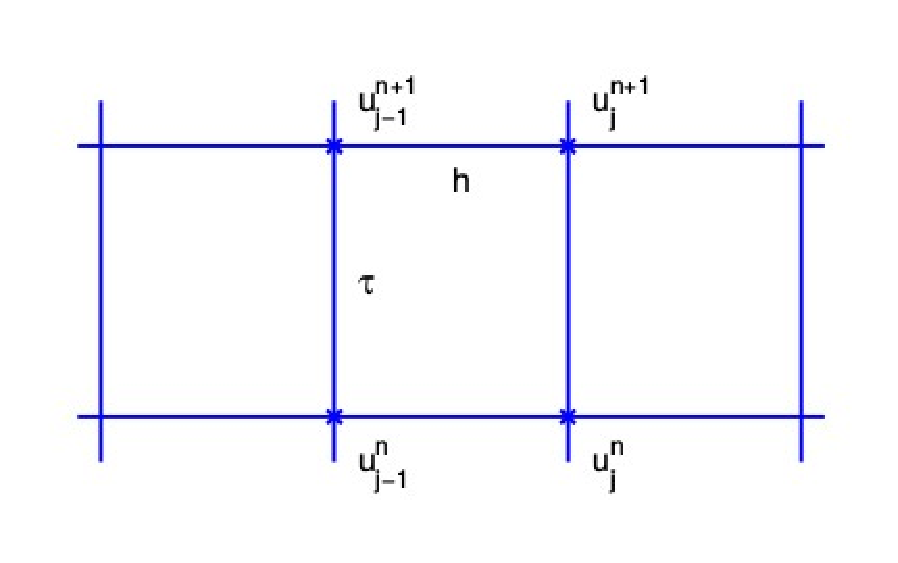
\includegraphics[height=4cm]{Figures/RCTFPM_mesh.eps}\\
	\caption[RCTFPM imaginary part]{}
\end{figure}



\begin{align*}
 u_{j}^{n+1} = \alpha_{-1}u_{j-1}^{n+1} + \beta_{-1}u_{j-1}^{n} + \beta_{0}u_{j}^{n}
\end{align*}

We expect the scheme to hold exactly for all the wave-formed functions in space.

\begin{align}
 V = {\{} v(x,t)|v(x,t) =  c_{1} + c_{2}\text{ exp}(ik_{j}(at-x)) + c_{3}\text{ exp}(-ik_{j}(at-x)), \hspace{0.5cm} \forall c_{1}, c_{2}, c_{3} \in \mathbb{C} {\}}  
\end{align}

where $k_{j}$ is the wave number in the j-th $[x_{j},x_{j+1}]$ cell and 'i' is the imaginary unit.
The complex-valued initial condition is denoted by $u_{0}(x)$. In the most general form it can be written as,
$u_{0}(x) = A_{0}(x)\text{exp}(iS_{0}(x))$, where $A_{0}(x)$ and $S_{0}(x)$ are real-valued functions.


We take the wave number as $k_{j} = S^{'}_{0}(x_{j})$ in each cell.

Taking the wave functions of $(c_{1}, c_{2}, c_{3}) = (1,0,0), (0,1,0), (0,0,1)$ in gives


\[ \begin{cases} 
      1 = \alpha_{-1} + \beta_{-1} + \beta_{0} \\
      \cos(k_{j}a\tau) = \alpha_{-1}\cos(k_{j}(a\tau+h)) +\beta_{-1} + \beta_{0}\\
      \sin(k_{j}a\tau) =  \alpha_{-1}\sin(k_{j}(a\tau+h)) - \beta_{-1}\sin(k_{j}h)\\
   \end{cases}
\]

By solving the above system we get,

\begin{align*}
 \alpha_{-1} &= \frac{\sin(k_{j}(a\tau-h)/2)}{\sin(k_{j}(a\tau+h)/2)}\\
 \beta_{-1} &= 1\\
 \beta_{0} &= -\alpha_{-1}
\end{align*}

\subsection{Stability Analysis}
We perform the Von Neumann Stability Analysis to get the stability criterion.
We susbtitute $u_{j}^{n}=e^{ij\xi h}$ and $u_{j}^{n+1} = G e^{ij\xi h}$ where G is the growth factor.
For the scheme to be stable we require
\begin{align*}
 |G| \leq 1
\end{align*}
Substituting in the scheme we get
\begin{align*}
 G e^{ij\xi h} &= \alpha_{-1}G e^{i(j-1)\xi h}+\beta_{-1} e^{i(j-1)\xi h}+\beta_{0} e^{ij\xi h}\\
 G &= \alpha_{-1}G e^{-i \xi h}+ e^{-i \xi h}-\alpha_{-1} \\
 (1-\alpha_{-1} e^{-i \xi h})G &= e^{-i \xi h}-\alpha_{-1}\\
 G &= \frac{e^{-i \xi h}-\alpha_{-1}}{1-\alpha_{-1} e^{-i \xi h}}\\ 
 \text{Taking absolute on both sides}\\
 |G| &= \Bigg{\lvert} \frac{e^{-i \xi h}-\alpha_{-1}}{1-\alpha_{-1} e^{-i \xi h}} \Bigg{\rvert}\\ \\
 |G| &= \frac{|e^{-i \xi h}-\alpha_{-1}|}{|1-\alpha_{-1} e^{-i \xi h}|}\\ \\
 |G| &= \frac{|\cos(\xi h) + i\sin(\xi h)-\alpha_{-1}|}{|1-\alpha_{-1} (\cos(\xi h) - i\sin(\xi h))|}\\ \\
 |G| &= \frac{|\cos(\xi h)-\alpha_{-1} + i\sin(\xi h)|}{|1-\alpha_{-1}\cos(\xi h) + i\alpha_{-1}\sin(\xi h)|}\\ \\
 |G| &= \sqrt{\frac{(\cos(\xi h)-\alpha_{-1})^2 + (\sin(\xi h))^2}{(1-\alpha_{-1}\cos(\xi h))^2 + (\alpha_{-1}\sin(\xi h))^2}}\\ \\
 |G| &= 1
\end{align*}
Thus the scheme is unconditionally stable.

This scheme is claimed to be second order in space.

\subsection{Example 1}
Consider the wave equation along with the given initial condition
\begin{align}
 \begin{split}
  u_{t} + u_{x} &= 0\\
   u(x,0) &= e^{-50x^2}e^{i\text{sin}(x)}
 \end{split} 
\end{align}
The analytical solution is given by
\begin{align}
 u(x,t) = e^{-50(x-t)^2}e^{i\text{sin}(x-t)}
\end{align}

The following plots and error estimates have been obtained on solving the above example using the tailored finite point method.\\

\begin{tabular}{|c|c|c|c|c|c|}
   \hline
   (h, $\tau$)  & (1/$2^{6}$,1/$2^{10}$)  & (1/$2^{7}$,1/$2^{10}$) & (1/$2^{8}$,1/$2^{10}$) &  (1/$2^{9}$,1/$2^{10}$)\\
  \hline
  Error  & 0.0293  & 0.0070 & 0.0016 &  0.0003\\
  \hline
  Order & -  &  2.05  & 2.08 & 2.32\\
\hline
\end{tabular}

\begin{figure}[htbp]
	\centering
		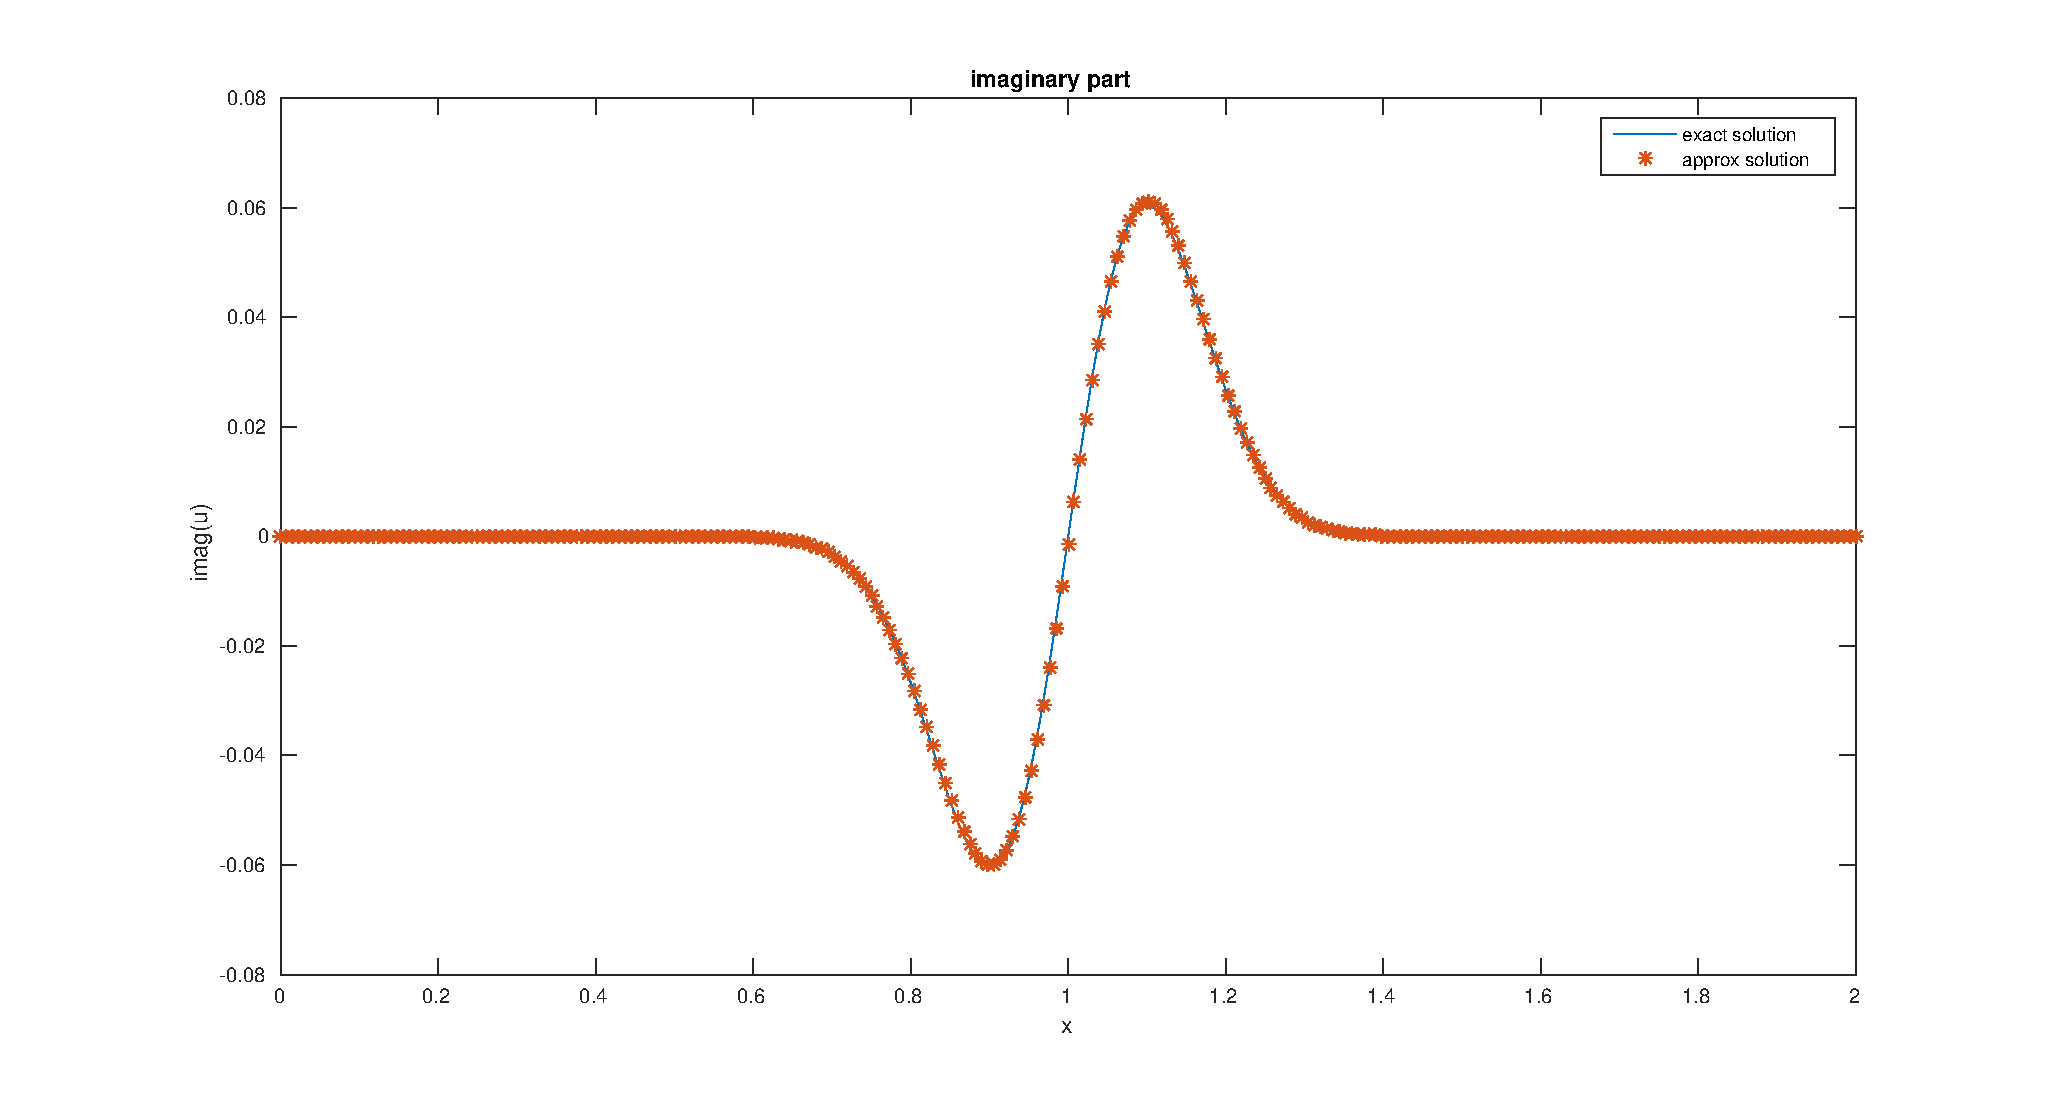
\includegraphics[height=8cm]{Figures/imag_RCTFPM2_2.eps}\\
		\rule{35em}{0.5pt}
	\caption[RCTFPM Real part]{}
\end{figure}

\begin{figure}[htbp]
	\centering
		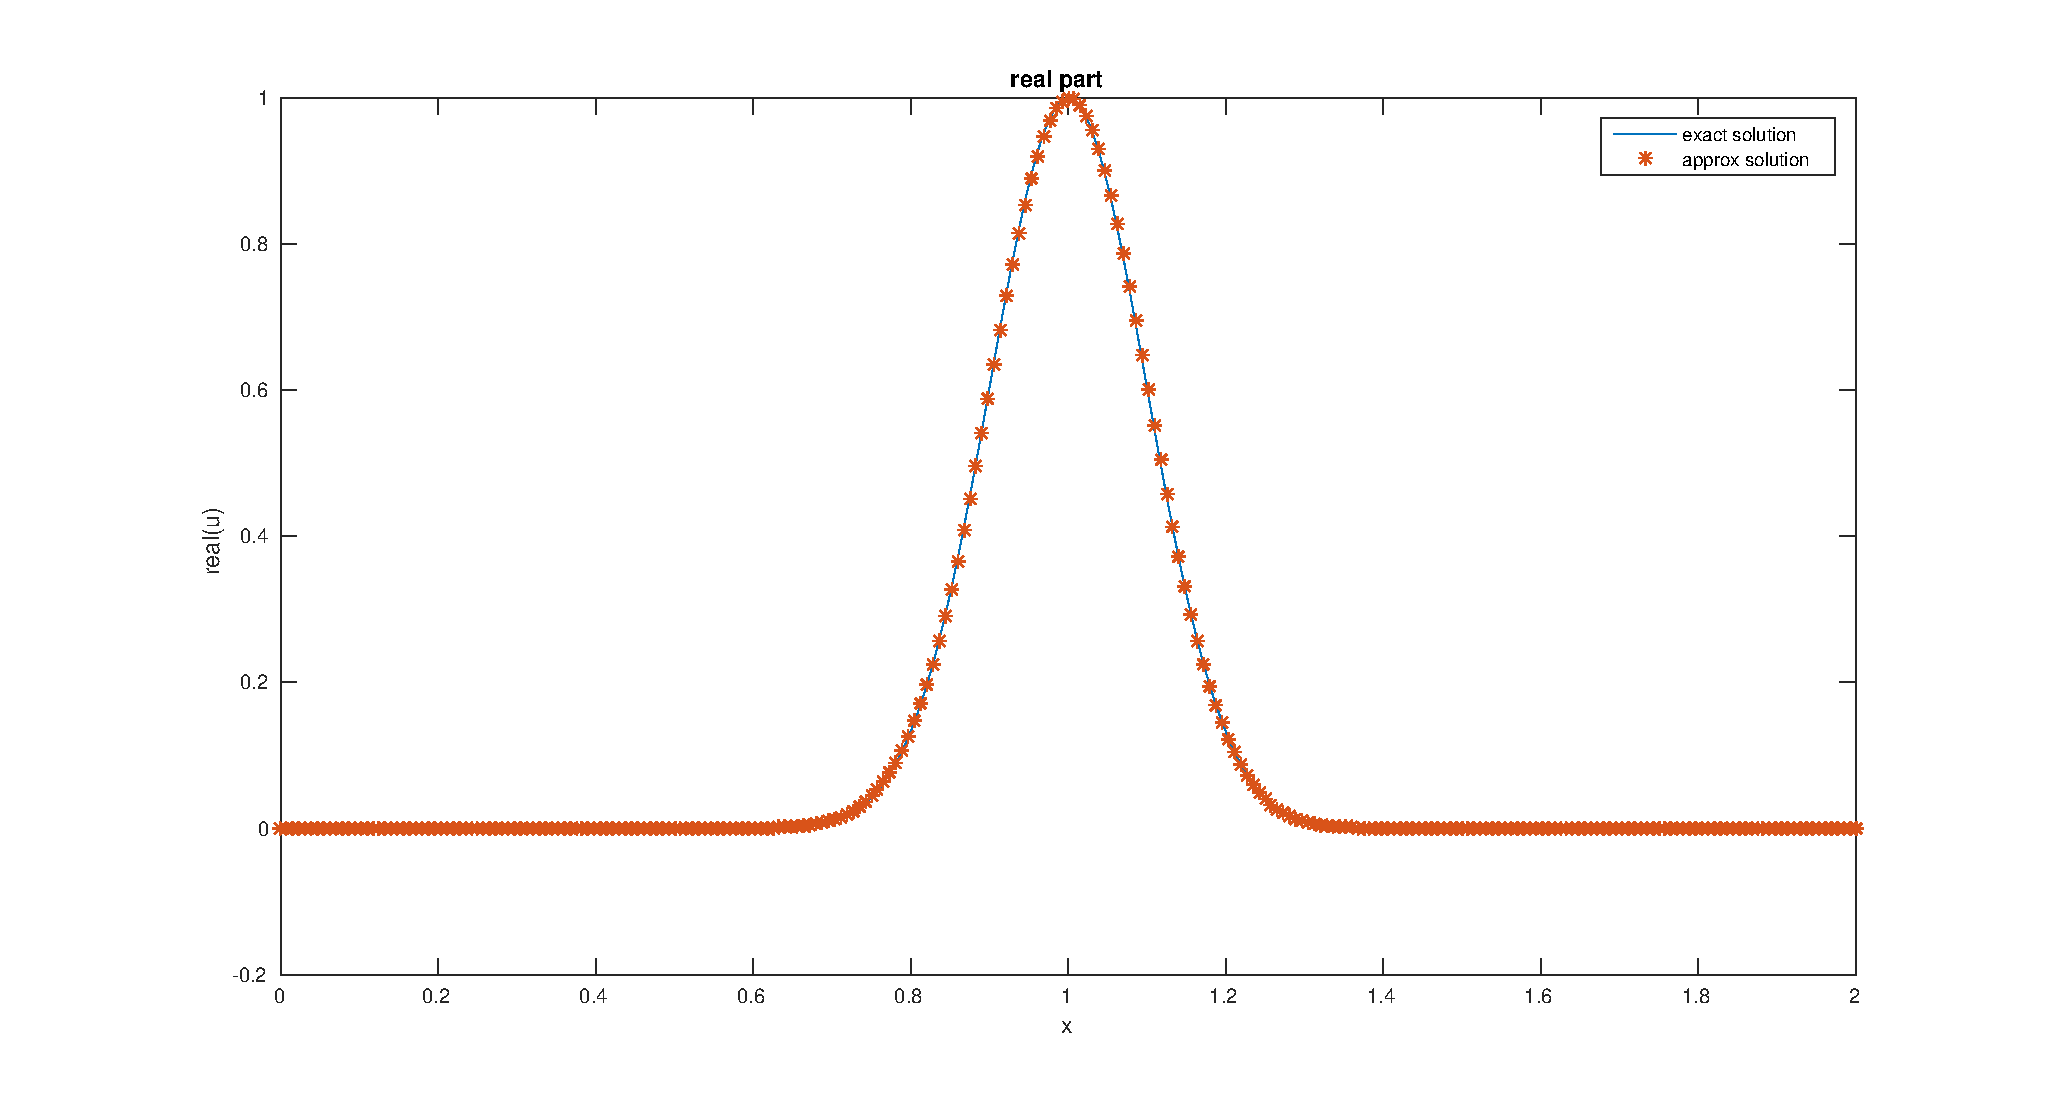
\includegraphics[height=8cm]{Figures/real_RCTFPM2_2.eps}\\
		\rule{35em}{0.5pt}
	\caption[RCTFPM imaginary part]{}
\end{figure}
\clearpage

\subsection{Example 2}
\begin{align}
 u_{t} + a(x)u_{x} = 0
\end{align}
The wave speed and initial condition are given as follows:
\begin{align}
 a(x) &= \pi + x\\
 u_{0}(x) &= e^{-50x^2}e^{i\sin(x)}
\end{align}
The exact solution is given by
\begin{align}
 u(x,t) = e^{-50((\pi+x)e^{-t}-\pi)^2}e^{(i\sin(\pi+x)e^{-t}-\pi)}
\end{align}
The wave number $k_{j}$ is taken to be $k_{j}=\cos(x_{j})$
Here we see that the wave speed is not a constant.
It is a linear function. The following approach is adopted when 'a' is not a constant:\\
We approximate $a(x)$ as
\begin{align}
 a(x) &\approx b_{j} + c_{j}x\hspace{5mm} \text{ where }\\
 b_{j} &= \frac{a(x_{j-1})x_{j}-a(x_{j})x_{j-1}}{h}
\end{align}
Then at the $n^{th}$ time step the solution can be locally approximated as
\begin{align}
 u(x_{j},t^{n}) = A_{0}(y_{j}^{n})e^{(iS_{0}(y_{j}^{n})/\epsilon)}
\end{align}
where
\begin{align}
 y_{j}^{n} = ((b_{j}+c_{j}x_{j})e^{-c_{j}t^{n}} -b_{j})/c_{j} 
\end{align}
We take the wave number as follows
\begin{align}
 k_{j}^{n} = S_{0}^{'}(y_{j}^{n})e^{-c_{n}t^{n}}/\epsilon
\end{align}

This example has been solved using the RCTFPM method. The following are the expressions for the coeffecients
\begin{align}
 \alpha_{-1}^{n} &= \frac{\sin(k_{j}^{n}(a_{j}\tau - h)/2)}{\sin(k_{j}^{n}(a_{j}\tau + h)/2)}\\
 \beta_{-1}^{n} &= 1\\
 \beta_{0}^{n} &= -\alpha_{-1}^{n}
\end{align}

The error estimates and plots obtained are given as follows:

\begin{tabular}{|c|c|c|c|c|c|}
   \hline
   (h, $\tau$)  & (1/$2^{6}$,1/$2^{10}$)  & (1/$2^{7}$,1/$2^{10}$) & (1/$2^{8}$,1/$2^{10}$) &  (1/$2^{9}$,1/$2^{10}$)\\
  \hline
  Error  & 0.0178  & 0.0058 & 0.0018 &  0.0007\\
  \hline
  Order & -  &  1.608  & 1.623 & 1.405\\
\hline
\end{tabular}

\begin{figure}[htbp]
	\centering
		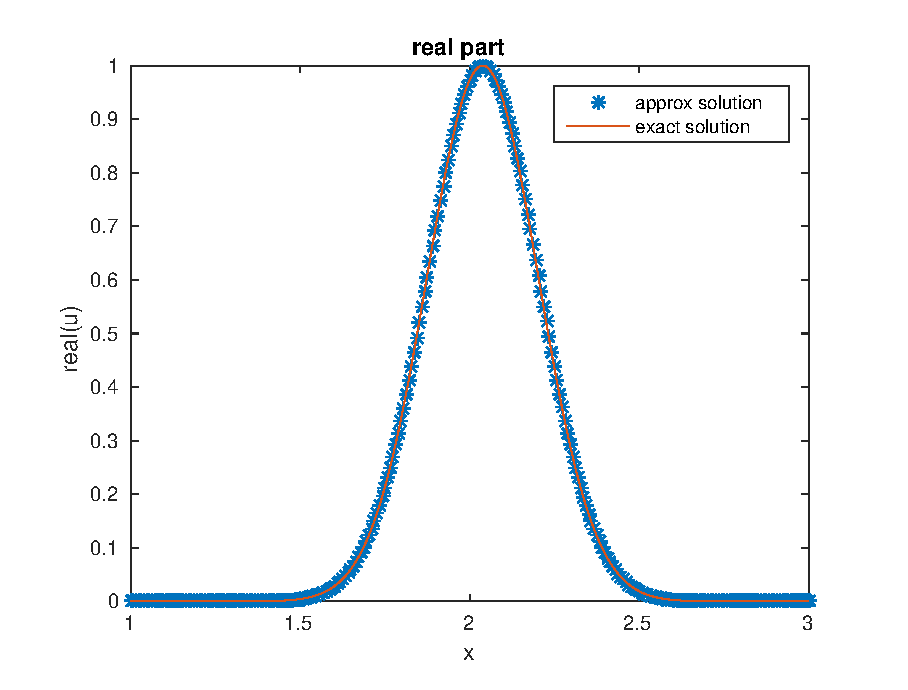
\includegraphics[height=8cm]{Figures/real_RCTFPM3_1.eps}\\
		\rule{35em}{0.5pt}
	\caption[RCTFPM Real part]{}
\end{figure}
\begin{figure}[htbp]
	\centering
		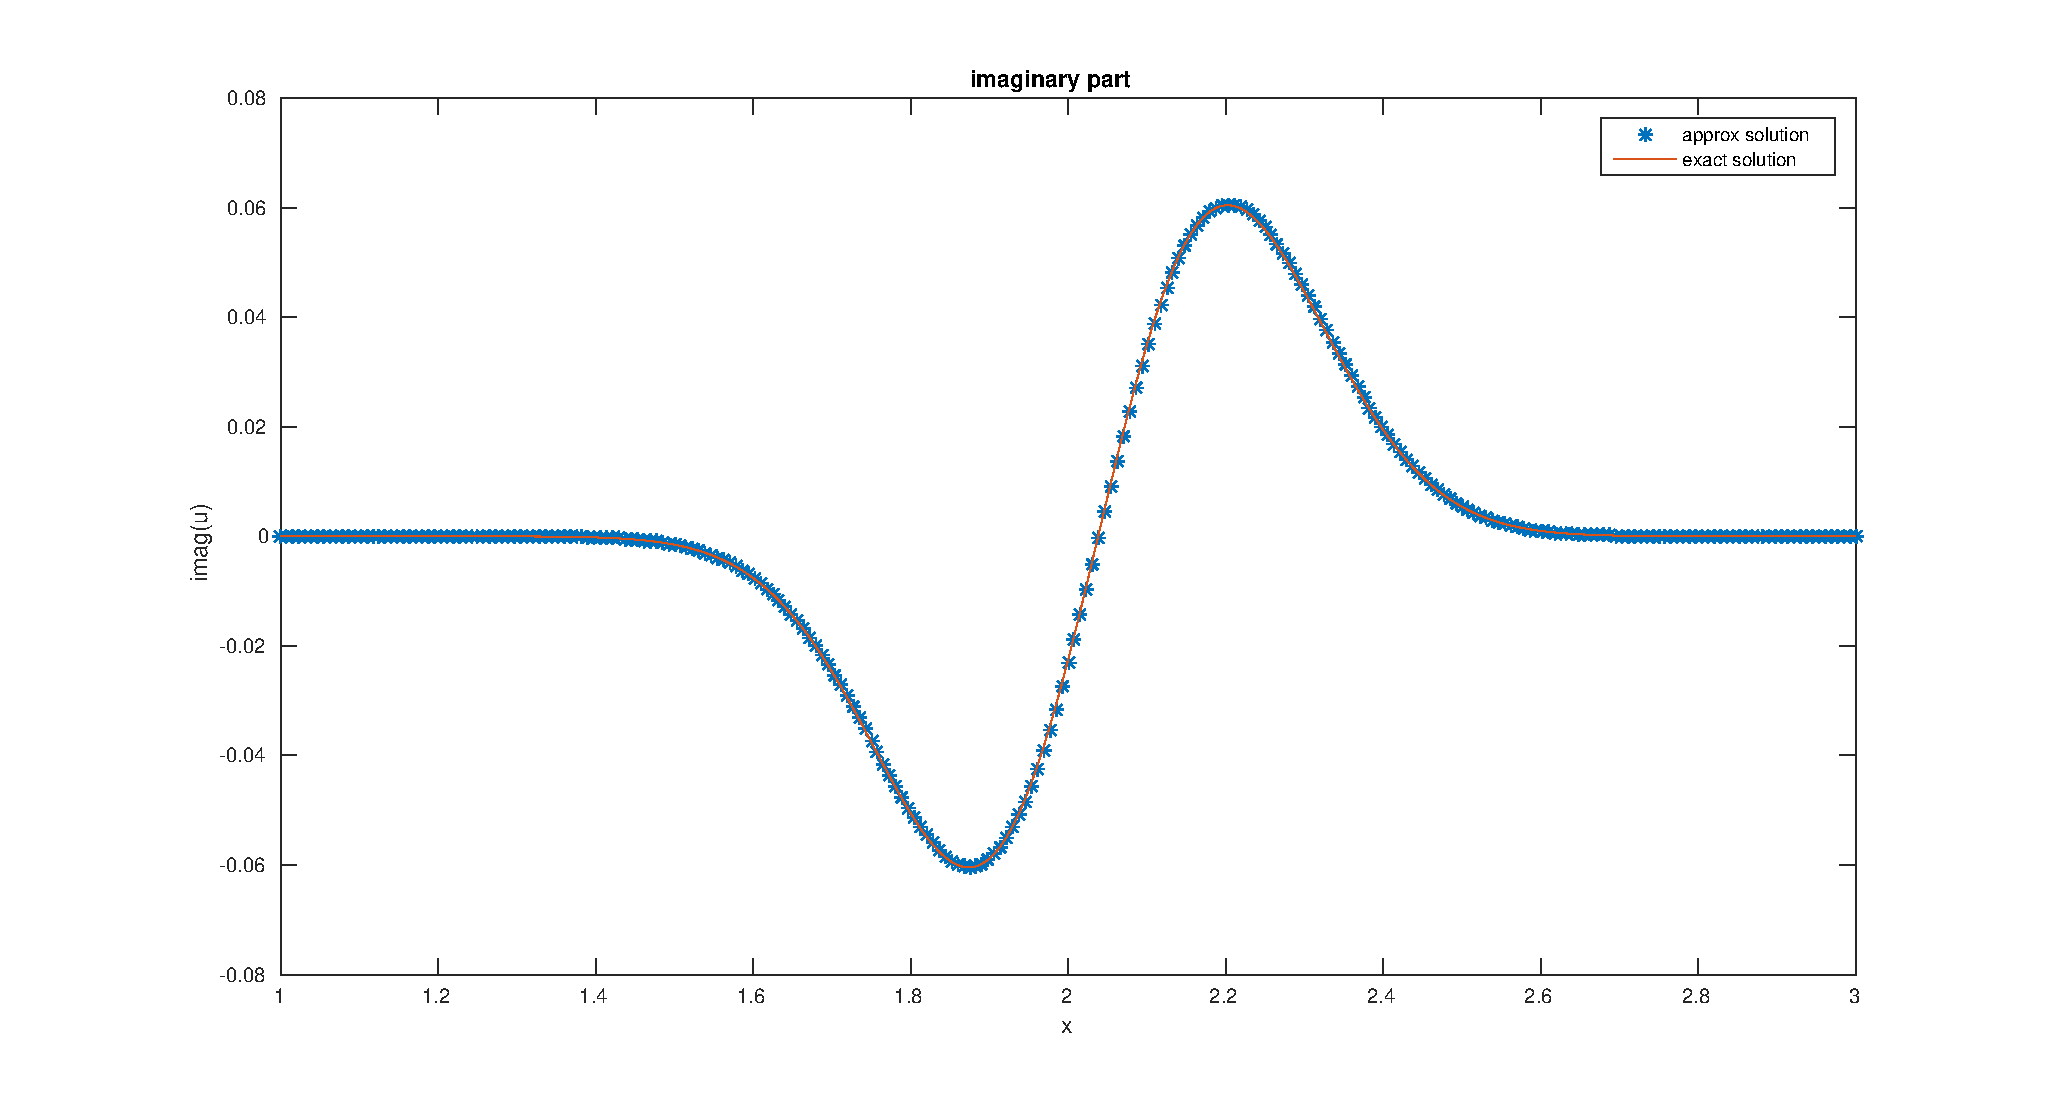
\includegraphics[height=8cm]{Figures/imag_RCTFPM3_1.eps}\\
		\rule{35em}{0.5pt}
	\caption[RCTFPM Real part]{}
\end{figure}
\clearpage
\subsection{Example 3}
\begin{align}
 u_{t} + a(x)u_{x} = 0
\end{align}
The wave speed and initial condition are given as follows:
\begin{align}
 a(x) &= 0.5 + x\\
 u_{0}(x) &= e^{-200x^2}e^{i\sin(x)/\epsilon}
\end{align}
The exact solution is given by
\begin{align}
 u(x,t) = e^{-50((\pi+x)e^{-t}-\pi)^2}e^{(i\sin(\pi+x)e^{-t}-\pi)}
\end{align}
The wave number $k_{j}$ is taken to be $k_{j}=\cos(x_{j})$

This example has been solved using the RCTFPM method.
The error estimates and plots obtained are given as follows:

\begin{tabular}{|c|c|c|c|c|c|}
   \hline
   (h, $\tau$)  & (1/$2^{7}$,1/$2^{6}$)  & (1/$2^{8}$,1/$2^{6}$) & (1/$2^{9}$,1/$2^{6}$) &  (1/$2^{10}$,1/$2^{6}$)\\
  \hline
  Error  & 0.0816  & 0.0381 & 0.0204 &  0.0105\\
  \hline
  Order & -  &  1.088  & 0.9102 & 0.9588\\
\hline
\end{tabular}

\begin{figure}[htbp]
	\centering
		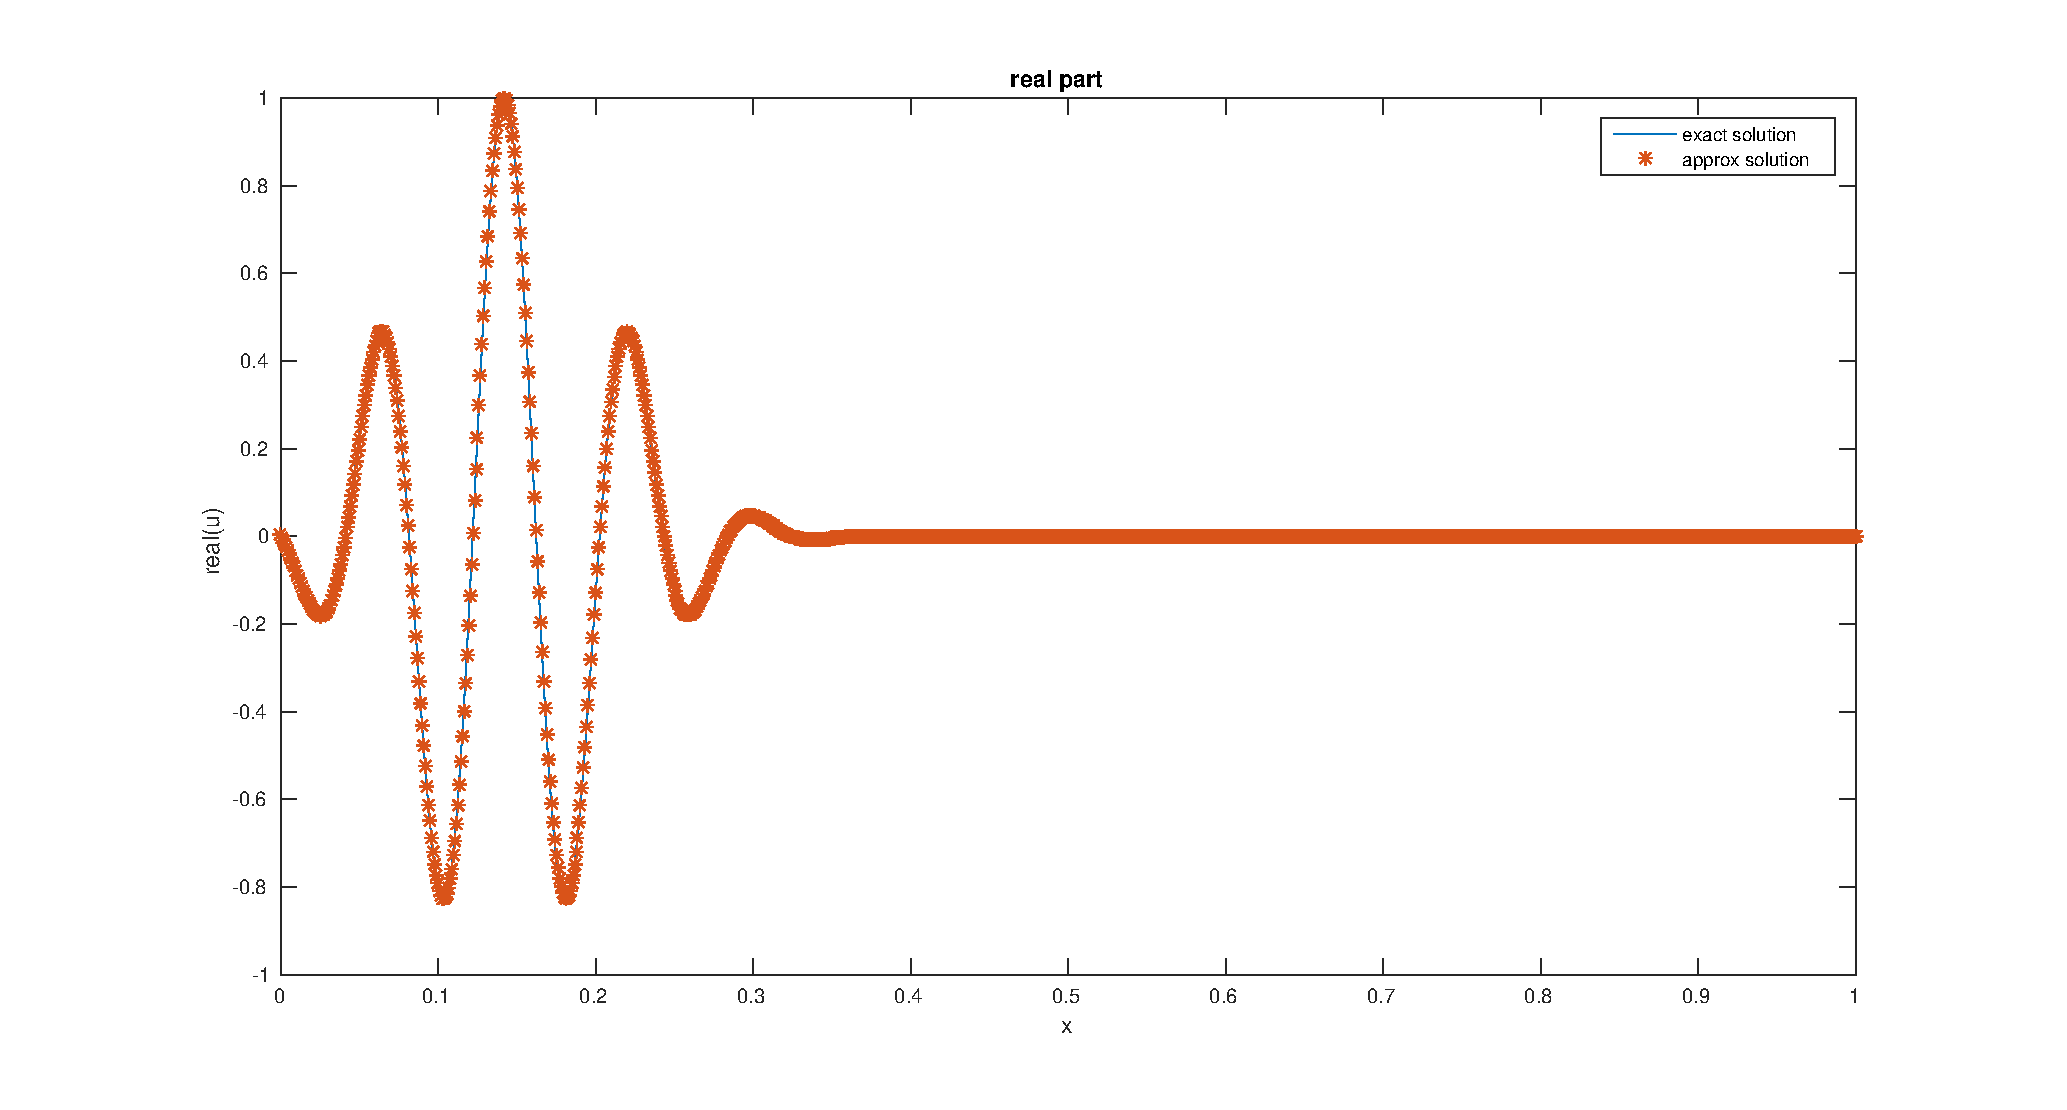
\includegraphics[height=8cm]{Figures/real_RCTFPM3_2.eps}\\
		\rule{35em}{0.5pt}
	\caption[RCTFPM Real part]{}
\end{figure}
\begin{figure}[htbp]
	\centering
		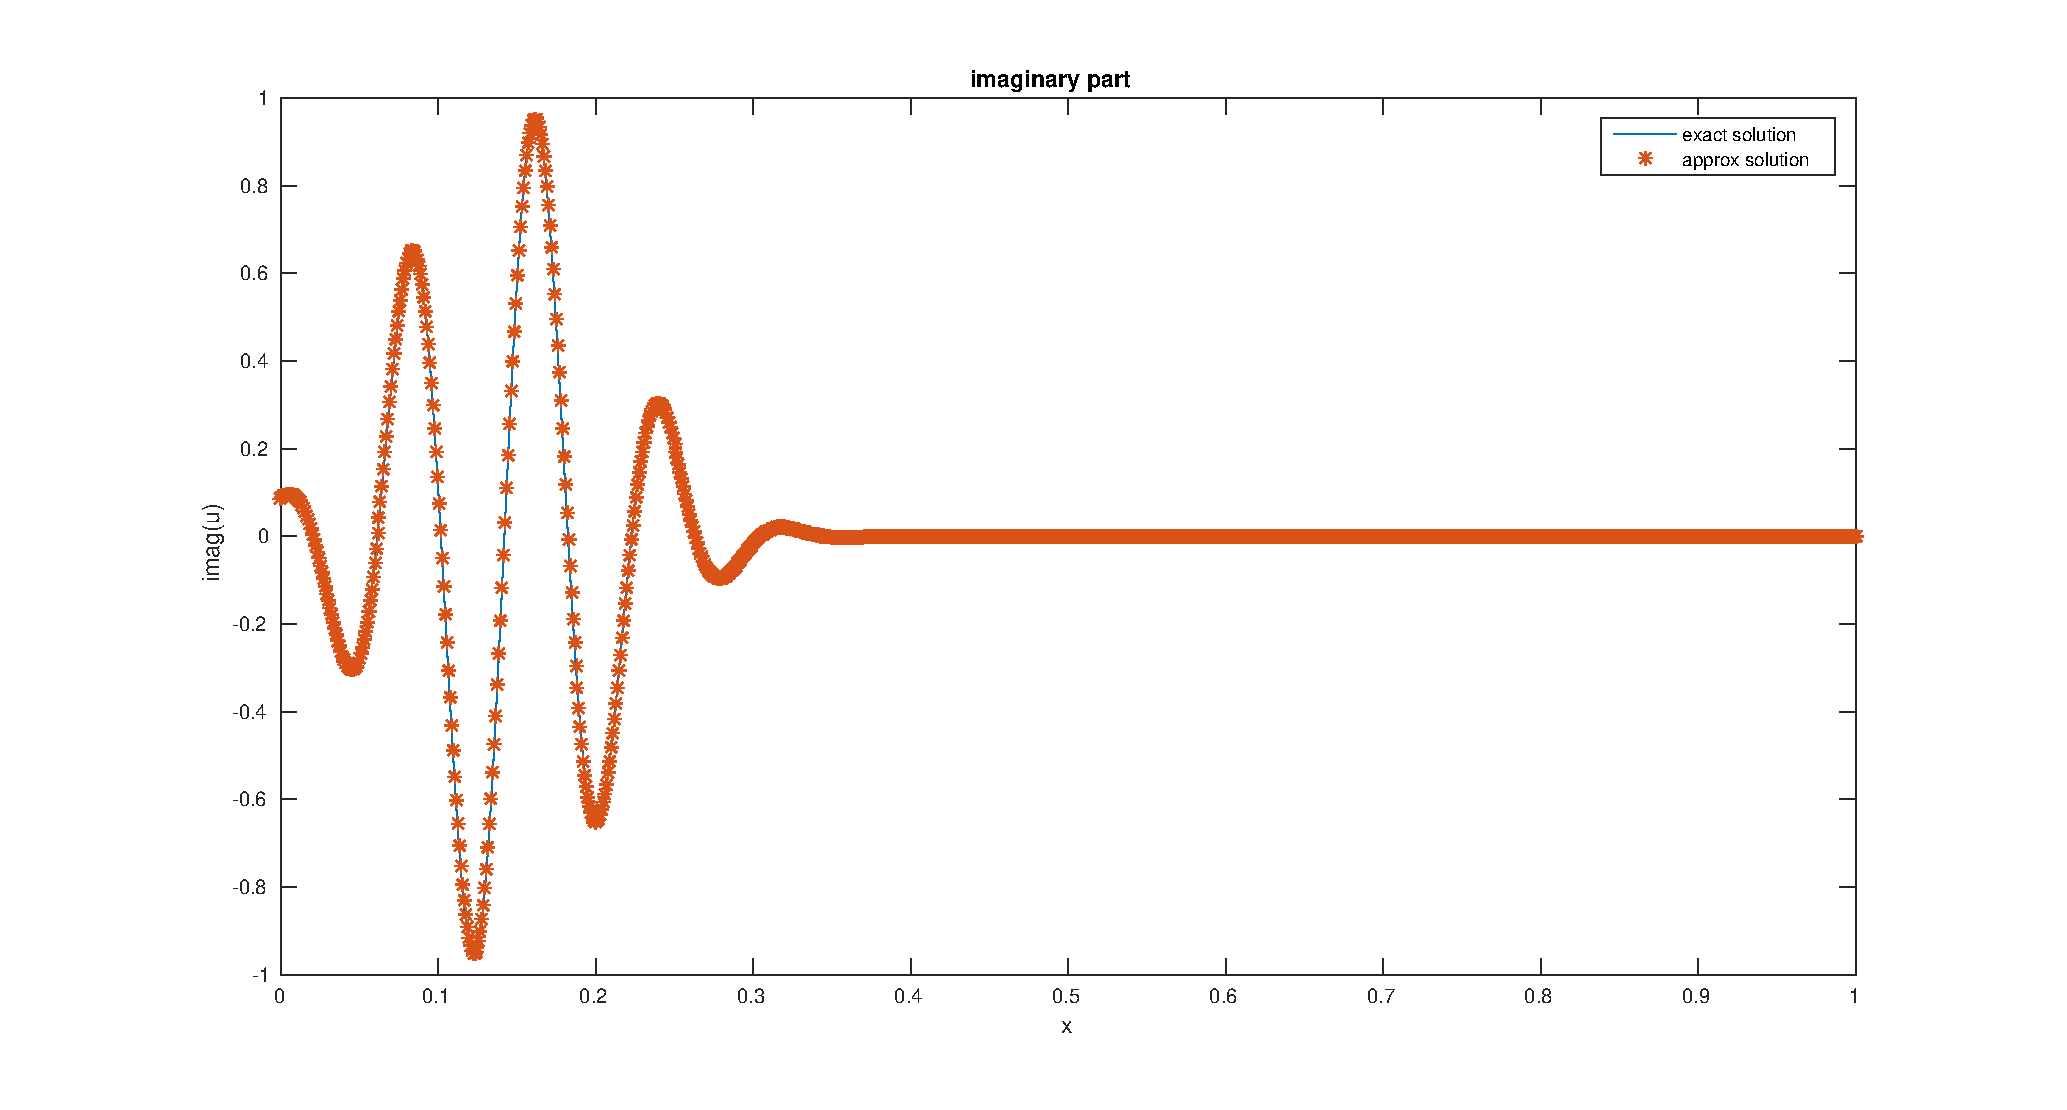
\includegraphics[height=8cm]{Figures/imag_RCTFPM3_2.eps}\\
		\rule{35em}{0.5pt}
	\caption[RCTFPM Real part]{}
\end{figure}
\clearpage

\section{Centered tailored finite point method (CTFPM)}
\begin{figure}[htbp]
	\centering
		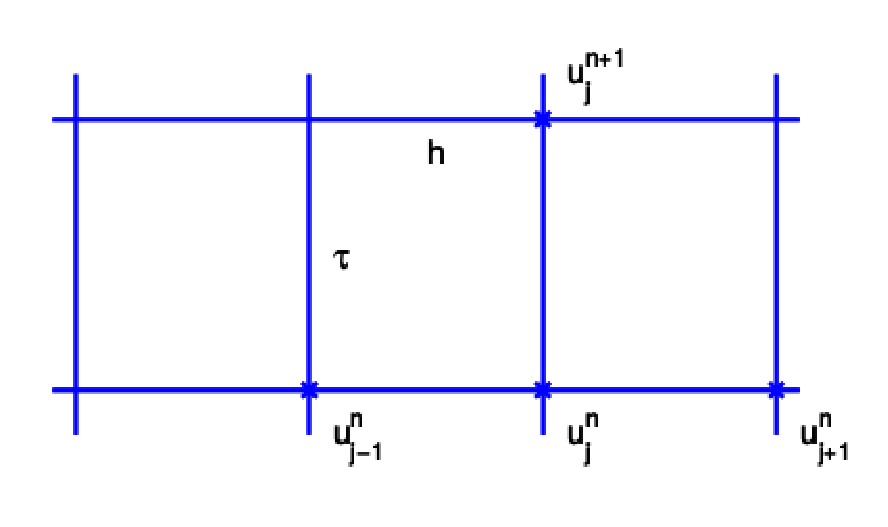
\includegraphics[height=4cm]{Figures/CTFPM_mesh.eps}\\
	\caption[RCTFPM imaginary part]{}
\end{figure}
We derive an explicit scheme as follows:

\begin{align}
u_{j}^{n+1} = \alpha_{-1}u_{j-1}^{n}+\alpha_{0}u_{j}^{n} + \alpha_{1}u_{j+1}^{n} 
\end{align}

The coefficients are taken as $(c_1,c_2,c_3) = (1,0,0),(0,1,0),(0,0,1)$ which gives us

\[ \begin{cases} 
      1 = \alpha_{-1} + \alpha_{0} + \alpha_{1} \\
      \cos(k_{j}a\tau) = \alpha_{-1}\cos(k_{j}h) +\alpha_{0} + \alpha_{1}\cos(k_{j}h)\\
      \sin(k_{j}a\tau) =  \alpha_{-1}\sin(k_{j}h) - \alpha_{1}\sin(k_{j}h)
   \end{cases}
\]

Solving this system yields,

\begin{align*}
 \alpha_{-1} =& \frac{\sin(k_{j}a\tau/2)\sin(k_{j}(a\tau + h)/2)}{\sin(k_{j}h/2)\sin(k_{j}h)}\\
 \alpha_{1} =& \frac{\sin(k_{j}a\tau/2)\sin(k_{j}(a\tau - h)/2)}{\sin(k_{j}h/2)\sin(k_{j}h)}\\
 \alpha_{0} =& 1 - \alpha{1} - \alpha_{-1}
\end{align*}

\subsection{Stability Analysis}
We perform the Von Neumann Stability Analysis to get the stability criterion.
Similar to the RCTFPM method we get,
\begin{align*}
 G = \alpha_{-1}e^{-i \xi h} + \alpha_{0} + \alpha_{1}e^{i \xi h}
\end{align*}
After calculating, the condition $|G| \leq 1$ is the same as
\begin{align*}
 1-\cos^2(k_{j}h)-\cos(k_{j}h) + \cos(k_{j} a \tau) + \cos(\xi h) - \cos(k_{j} h)\cos(k_{j} a \tau ) \cos(\xi h) \geq 0 \\
 (1+\cos(\xi h))(1-\cos(k_{j} h) \cos(k_{j} a \tau)) + (1+ \cos(k_{j} h))(\cos(k_{j} a \tau) - \cos(k_{j} h)) \geq 0
\end{align*}
As $k_{j} a \tau, k_{j} h << 1$.
Thus for the scheme to be stable we require $a \tau \leq h$.\\

\subsection{Accuracy}
We use the taylor series expansion to see the accuracy of the scheme.
Consider the terms
\begin{align*}
 u_{j-1}^{n} &\approx u(x-h,t) \approx u(x,t)-hu_{x}(x,t) + \frac{h^2}{2}u_{xx}(x,t)+o(h^3)\\
 u_{j+1}^{n} &\approx u(x+h,t) \approx u(x,t)+hu_{x}(x,t) + \frac{h^2}{2}u_{xx}(x,t)+o(h^3)\\
 u_{j}^{n} &\approx u(x,t)
\end{align*}
Substituting the above expressions in the  L.H.S of (1.22). We get
\begin{align*}
 &=\alpha_{-1}(u(x,t)-hu_{x}(x,t) + \frac{h^2}{2}u_{xx}(x,t))+\alpha_{0}(u(x,t)) + \alpha_{1}( u(x,t)+hu_{x}(x,t) + \frac{h^2}{2}u_{xx}(x,t))\\
 &=(\alpha_{-1}+\alpha_{0}+\alpha_{1})u(x,t) + h(\alpha_{1}-\alpha_{-1})u_{x}(x,t)+\frac{h^2}{2}(\alpha_{1}+\alpha_{-1})u_{xx}(x,t)\\
 &=u(x,t)+h(\alpha_{1}-\alpha_{-1})u_{x}(x,t)+\frac{h^2}{2}(\alpha_{1}+\alpha_{-1})u_{xx}(x,t)
\end{align*}
In th discrete form
\begin{align*}
 &=u_{j}^{n}+h((\alpha_{1}-\alpha_{-1})\frac{(u_{j+1}^{n}-u_{j-1}^{n})}{2h})+\frac{h^2}{2}(\alpha_{1}+\alpha_{-1})\frac{u_{j-1}^{n}-2u_{j}^{n}+u_{j+1}^{n}}{h^2}
\end{align*}
From calculating we have
\begin{align*}
 \alpha_{1}-\alpha_{-1}&= -\frac{\sin(k_{j}a\tau)}{\sin(k_{j} h)}\\
 \alpha_{1}+\alpha_{-1}&= \frac{\sin^2((k_{j}a\tau)/2)}{\sin^2((k_{j} h)/2)}
\end{align*}
As $k_j a\tau $,\hspace{2mm} $k_{j}h <<1$. We have
\begin{align*}
 \alpha_{1}-\alpha_{-1}&= -\frac{a\tau}{h}\\
 \alpha_{1}+\alpha_{-1}&= \frac{(a\tau)^2}{h^2}
\end{align*}
Substituting above we get,
\begin{align*}
 &=u_{j}^{n}-\frac{(a\tau)}{2h} (u_{j+1}^{n}-u_{j-1}^{n})+\frac{(a\tau)^2}{2h^2} (u_{j-1}^{n}-2u_{j}^{n}+u_{j+1}^{n})
\end{align*}
Equating with R.H.S we get

\begin{align*}
 u_{j}^{n+1} = u_{j}^{n} - \frac{a \tau}{2h} (u_{j+1}^{n}-u_{j-1}^{n}) + (a \tau)^2\bigg{(}\frac{u_{j-1}^{n}-2u_{j}^{n}+u_{j+1}^{n}}{2h^2}\bigg{)}
\end{align*}

This is the Lax Wendroff scheme which is second order accurate.

This scheme is second order in space.


\subsection{Example}
Consider the wave equation along with the given initial condition
\begin{align}
 \begin{split}
  u_{t} + u_{x} &= 0\\
   u(x,0) &= e^{-50x^2}e^{i\text{sin}(x)}
 \end{split} 
\end{align}
The analytical solution is given by
\begin{align}
 u(x,t) = e^{-50(x-t)^2}e^{i\text{sin}(x-t)}
\end{align}

The following plots and error estimates have been obtained on solving the above example using the tailored finite point method.\\

\vspace{2cm}

\begin{tabular}{|c|c|c|c|c|c|}
   \hline
   (h, $\tau$)  & (1/$2^{6}$,1/$2^{7}$)  & (1/$2^{7}$,1/$2^{8}$) & (1/$2^{8}$,1/$2^{9}$) &  (1/$2^{9}$,1/$2^{10}$)\\
  \hline
  Error  & 0.03996  & 0.01049 & 0.00265 &  6.65558e-04\\
  \hline
  Order & -  &  1.92  & 1.98 & 1.99\\
\hline
\end{tabular}

\begin{figure}[htbp]
	\centering
		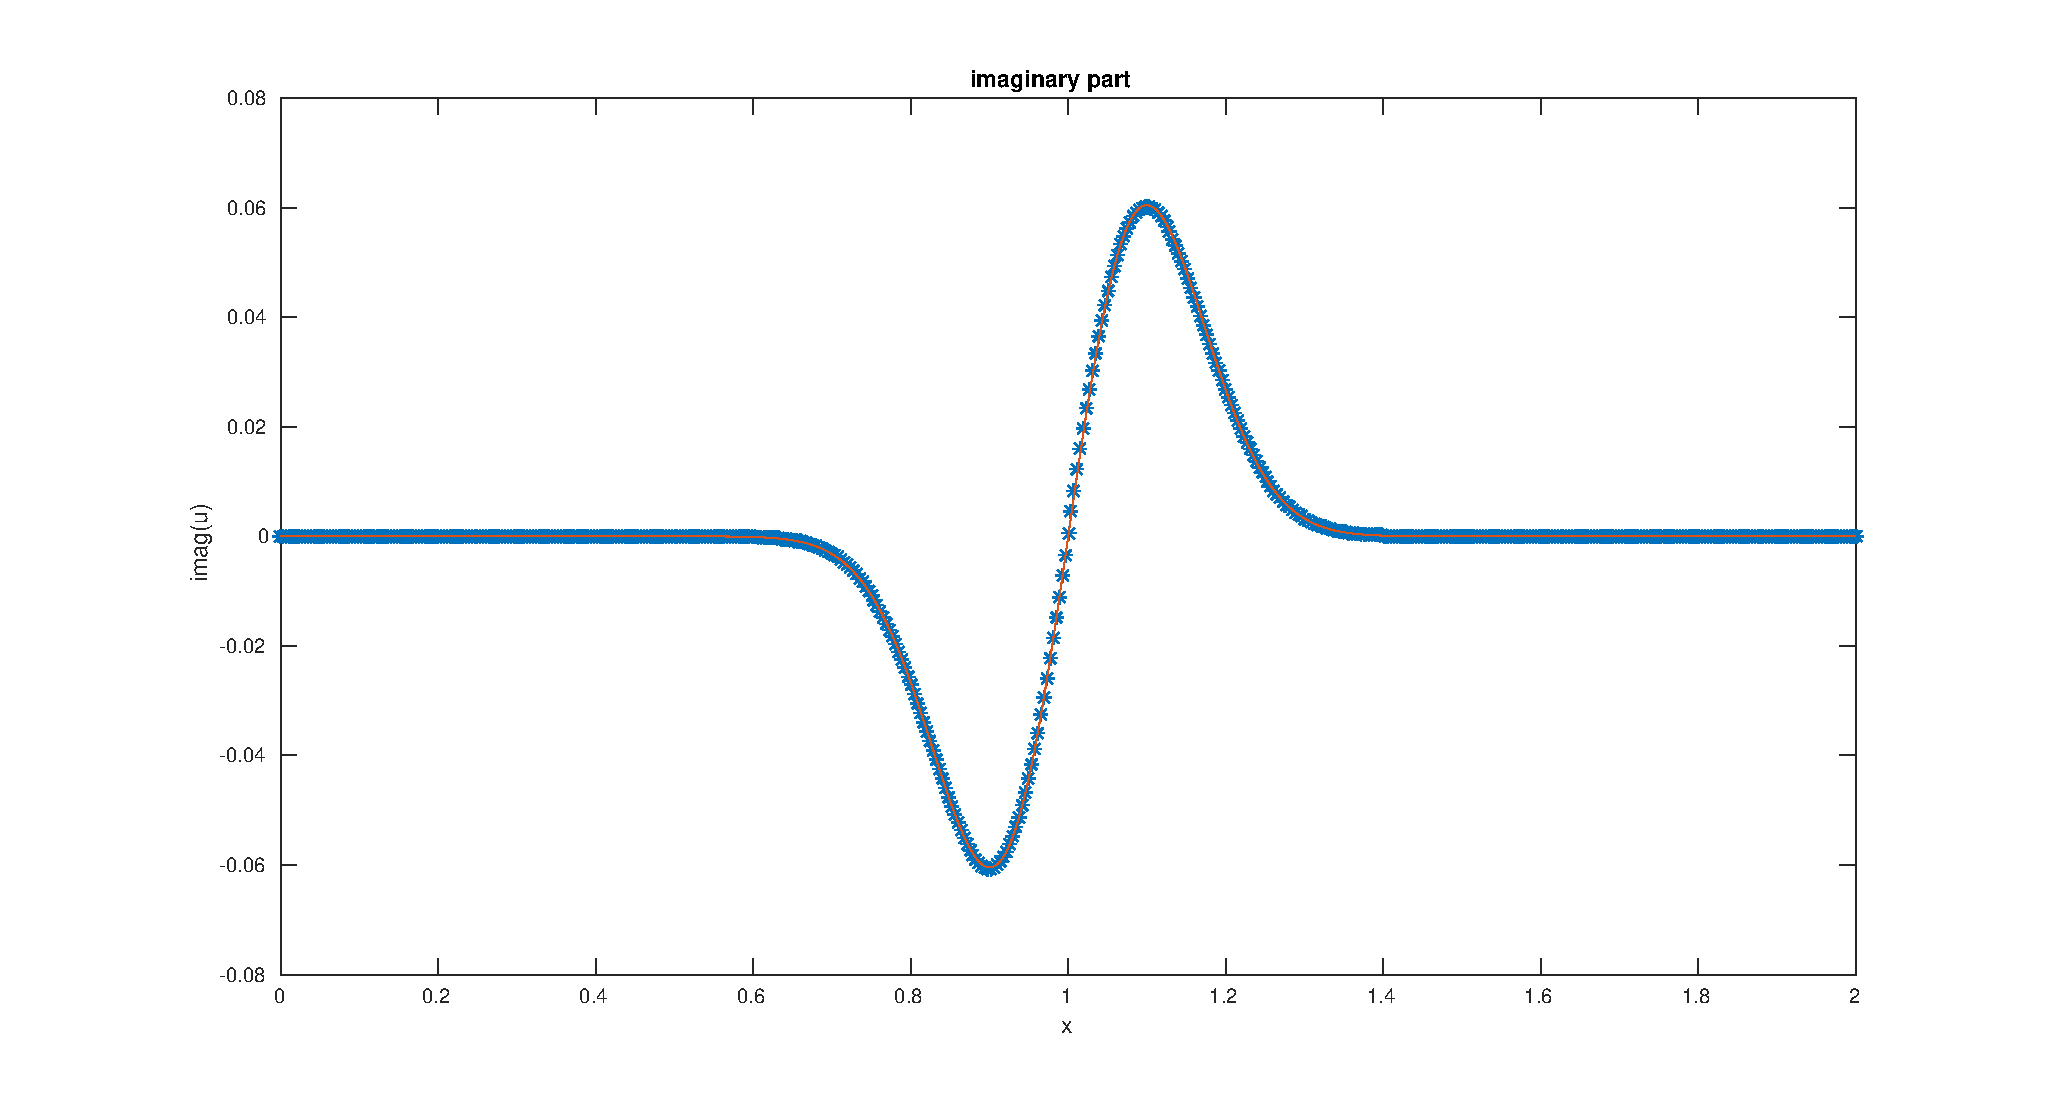
\includegraphics[height=8cm]{Figures/imag_CTFPM.eps}\\
		\rule{35em}{0.5pt}
	\caption[RCTFPM Real part]{}
\end{figure}

\begin{figure}[htbp]
	\centering
		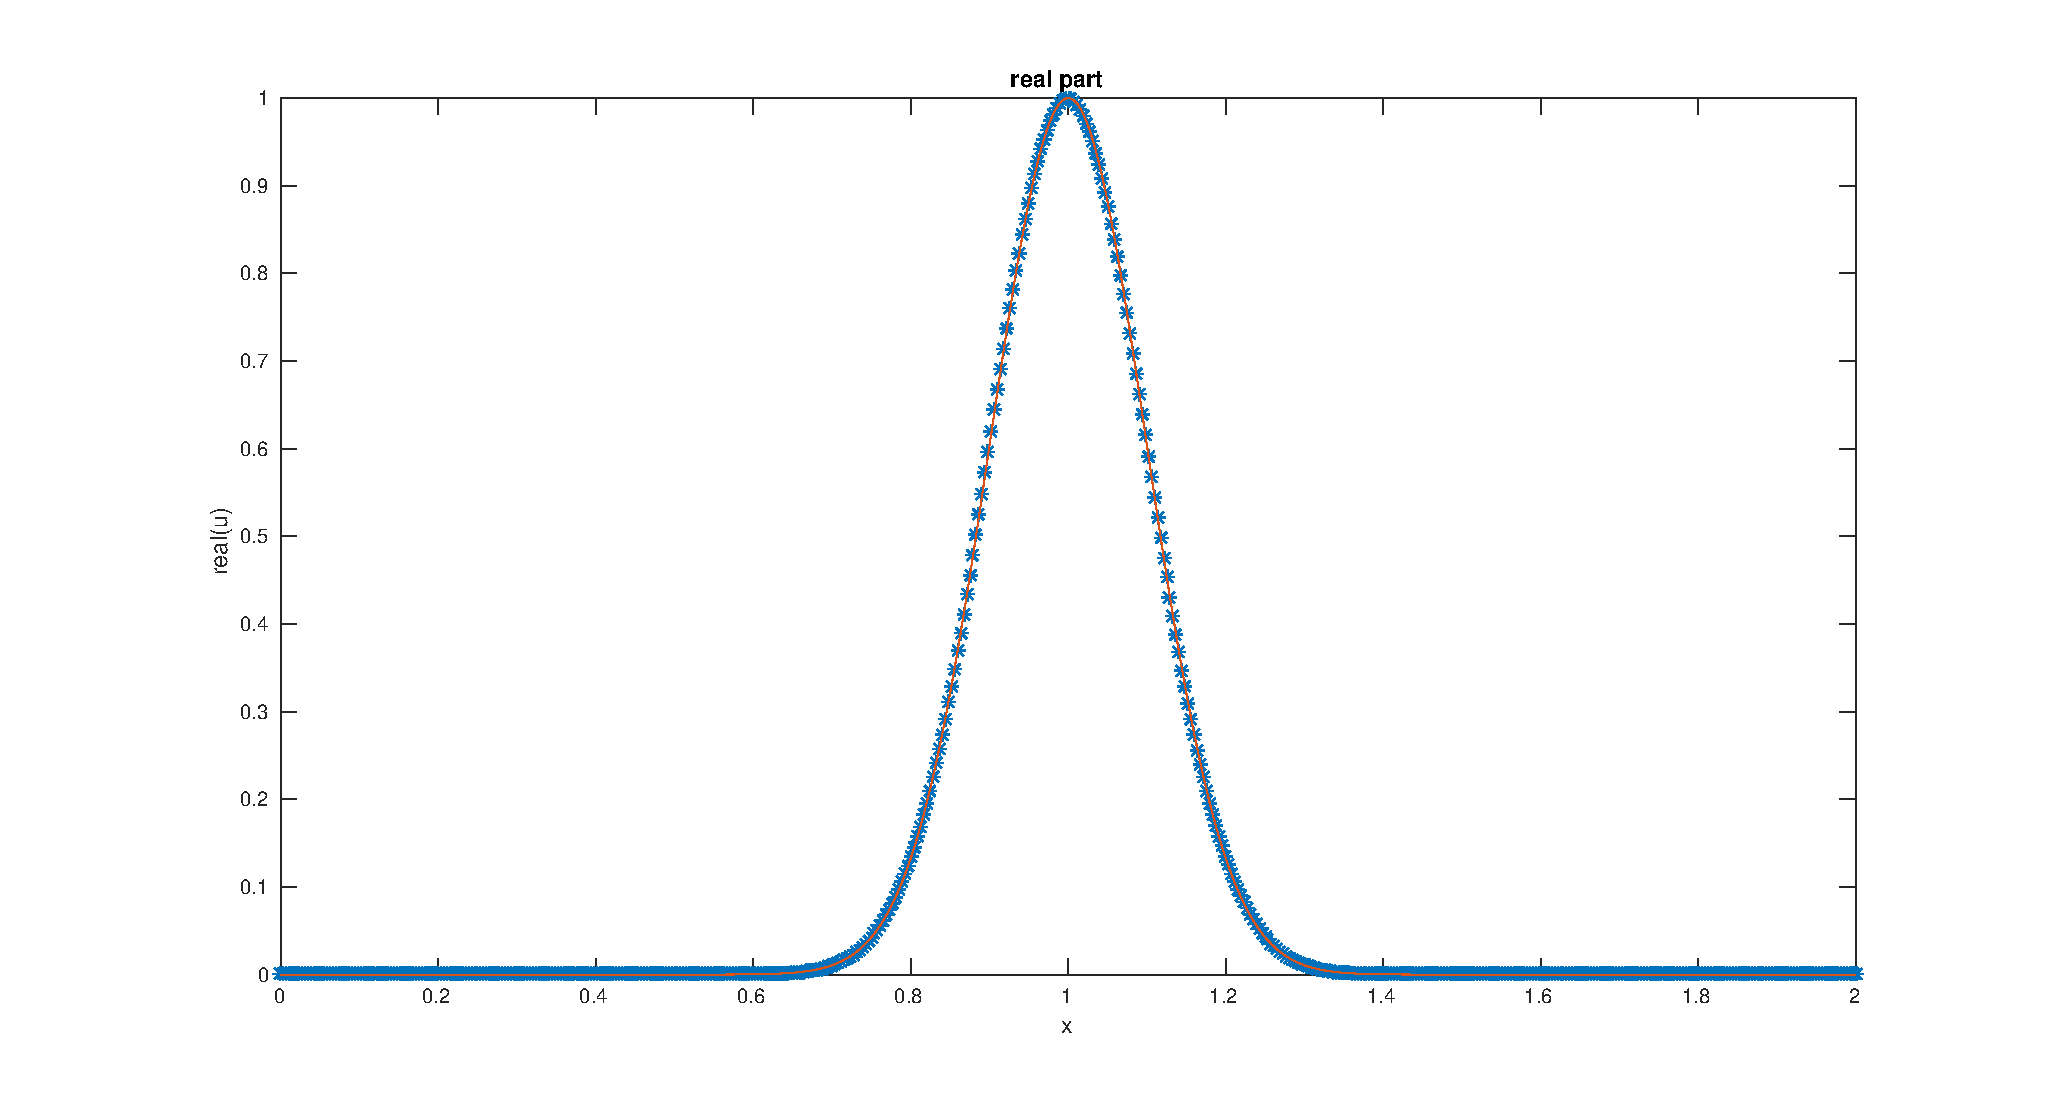
\includegraphics[height=8cm]{Figures/real_CTFPM.eps}\\
		\rule{35em}{0.5pt}
	\caption[RCTFPM imaginary part]{}
\end{figure}


\clearpage

\section{One Sided Tailored Finite Point Method (OSTFPM)}
\begin{figure}[htbp]
	\centering
		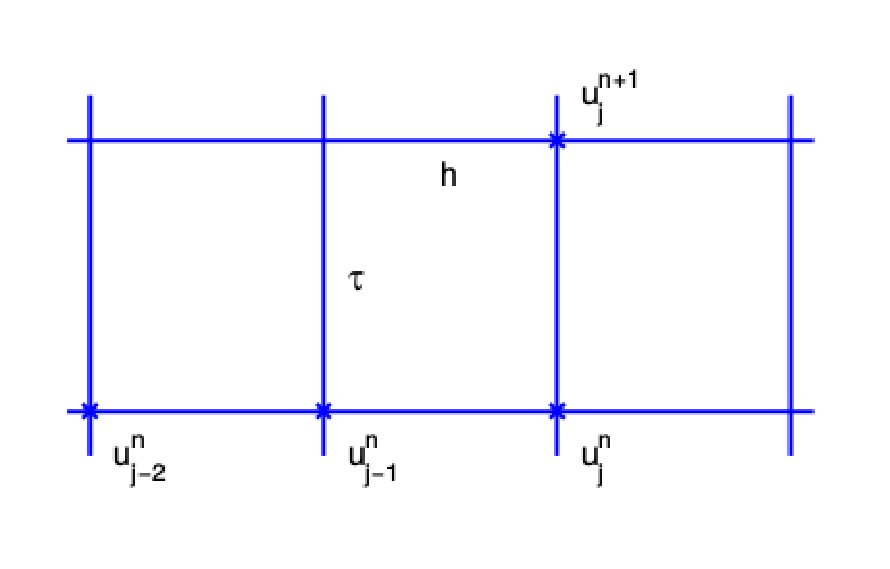
\includegraphics[height=4cm]{Figures/OSTFPM_mesh.eps}\\
	\caption[RCTFPM imaginary part]{}
\end{figure}
Many a times for boundary value problems the OSTFPM is an efficient method.The scheme is given as follows:
\begin{align}
 u_{j}^{n+1} = \alpha_{-2}u_{j-2}^{n} + \alpha_{-1}u_{j-1}^{n} + \alpha_{0}u_{j}^{n}
\end{align}

The coefficients are taken as $(c_1,c_2,c_3) = (1,0,0),(0,1,0),(0,0,1)$ which gives us

\[ \begin{cases} 
      1 = \alpha_{-2} + \alpha_{-1} + \alpha_{0} \\
      \cos(k_{j}a\tau) = \alpha_{-2}\cos(2k_{j}h) +\alpha_{-1}\cos(k_{j} h) + \alpha_{0}\\
      \sin(k_{j}a\tau) =  \alpha_{-2}\sin(2k_{j}h) + \alpha_{-1}\sin(k_{j}h)\\
   \end{cases}
\]
this gives us

\begin{align*}
 \alpha_{-2} &= \frac{\sin(k_{j}a\tau /2)\sin(k_{j}(a\tau - h)/2)}{\sin(k_{j}h/2)\sin(k_{j}h)}\\
 \alpha_{-1} &= \frac{\sin(k_{j}a\tau /2)\sin(k_{j}(a\tau - 2h)/2)}{\sin^2(k_{j}h/2)}\\
 \alpha_{0} &= 1-\alpha_{-2}-\alpha_{-1}
\end{align*}

\subsection{Stability Criterion}
%We perform the Von Neumann Stability Analysis to get the stability criterion.
The stability criterion of the scheme is a better than CTFPM. For the scheme to be stable we require
$\tau \leq 2h $.\\
%\begin{align*}
% G e^{i j \xi h} &= \alpha_{-2} e^{i (j-2) \xi h} + \alpha_{-1}e^{i (j-1) \xi h} + \alpha_{0}e^{i j \xi h}\\
% G &= \alpha_{-2} e^{-2 i \xi h} + \alpha_{-1} e^{-i \xi h} + \alpha_{0}
%\end{align*}
%On solving the above equation we require $a \tau \leq 2h$ for the scheme to be stable.
This scheme is second order in space.

\subsection{Accuracy}
\begin{align*}
 & u_{j-2}^{n} \approx u(x-2,t) \approx u(x,t) - 2h u_{x}(x,t) +2h^2 u_{xx}(x,t) + o(h^3)\\
 & u_{j-1}^{n} \approx u(x-1,t) \approx u(x,t) -h u_{x} + \frac{h^2}{2} u_{xx}(x,t) +o(h^3)\\
 & u_{j}^{n} \approx u(x,t)
\end{align*}

Substituting these values in the scheme, we get
\begin{align*}
 &= \alpha_{-2}(u-2hu_{x}+2h^2u_{xx}) + \alpha_{-1}(u-hu_{x}+\frac{h^2}{2}) + \alpha_{0}u_{j}^{n}\\
 &= (\alpha_{-2}+\alpha_{-1}+\alpha_{0})u - h(2 \alpha_{-2} + \alpha_{-1})u_{x} + h^2(\frac{\alpha_{-1}}{2}+2 \alpha_{-2}) u_{xx}\\
 &= u - h(\alpha_{-2}+\alpha_{-1})u_{x} + h^2 (2 \alpha_{-2} + \alpha_{-1}/2) u_{xx}\\
 &= u-a\tau u_{x} + \frac{(a \tau)^2}{2}u_{xx}\\
\end{align*}

In discrete form

\begin{align*}
 u_{j}^{n} - \frac{a \tau}{2h} (u_{j+1}^{n}-u_{j-1}^{n}) + \frac{(a \tau)^2}{2}\bigg{(}\frac{u_{j-1}^{n}-2u_{j}^{n}+u_{j+1}^{n}}{h^2}\bigg{)}
\end{align*}
Equating with R.H.S we get

\begin{align*}
 u_{j}^{n+1} = u_{j}^{n} - \frac{a \tau}{2h} (u_{j+1}^{n}-u_{j-1}^{n}) + \frac{(a \tau)^2}{2h^2}(u_{j-1}^{n}-2u_{j}^{n}+u_{j+1}^{n})
\end{align*}

This is the Lax Wendroff scheme which is second order accurate.

\subsection{Example}
Consider the wave equation along with the given initial condition
\begin{align}
 \begin{split}
  u_{t} + u_{x} &= 0\\
   u(x,0) &= e^{-50x^2}e^{i\text{sin}(x)}
 \end{split} 
\end{align}
The analytical solution is given by
\begin{align}
 u(x,t) = e^{-50(x-t)^2}e^{i\text{sin}(x-t)}
\end{align}

The following plots and error estimates have been obtained on solving the above example using the tailored finite point method.\\

\begin{tabular}{|c|c|c|c|c|c|}
   \hline
   (h, $\tau$)  & (1/$2^{6}$,1/$2^{7}$)  & (1/$2^{7}$,1/$2^{8}$) & (1/$2^{8}$,1/$2^{9}$) &  (1/$2^{9}$,1/$2^{10}$)\\
  \hline
  Error  & 0.1203  & 0.0434 & 0.0153 &  0.0054\\
  \hline
  Order & -  &  1.47  & 1.50 & 1.49\\
\hline
\end{tabular}


\begin{figure}[htbp]
	\centering
		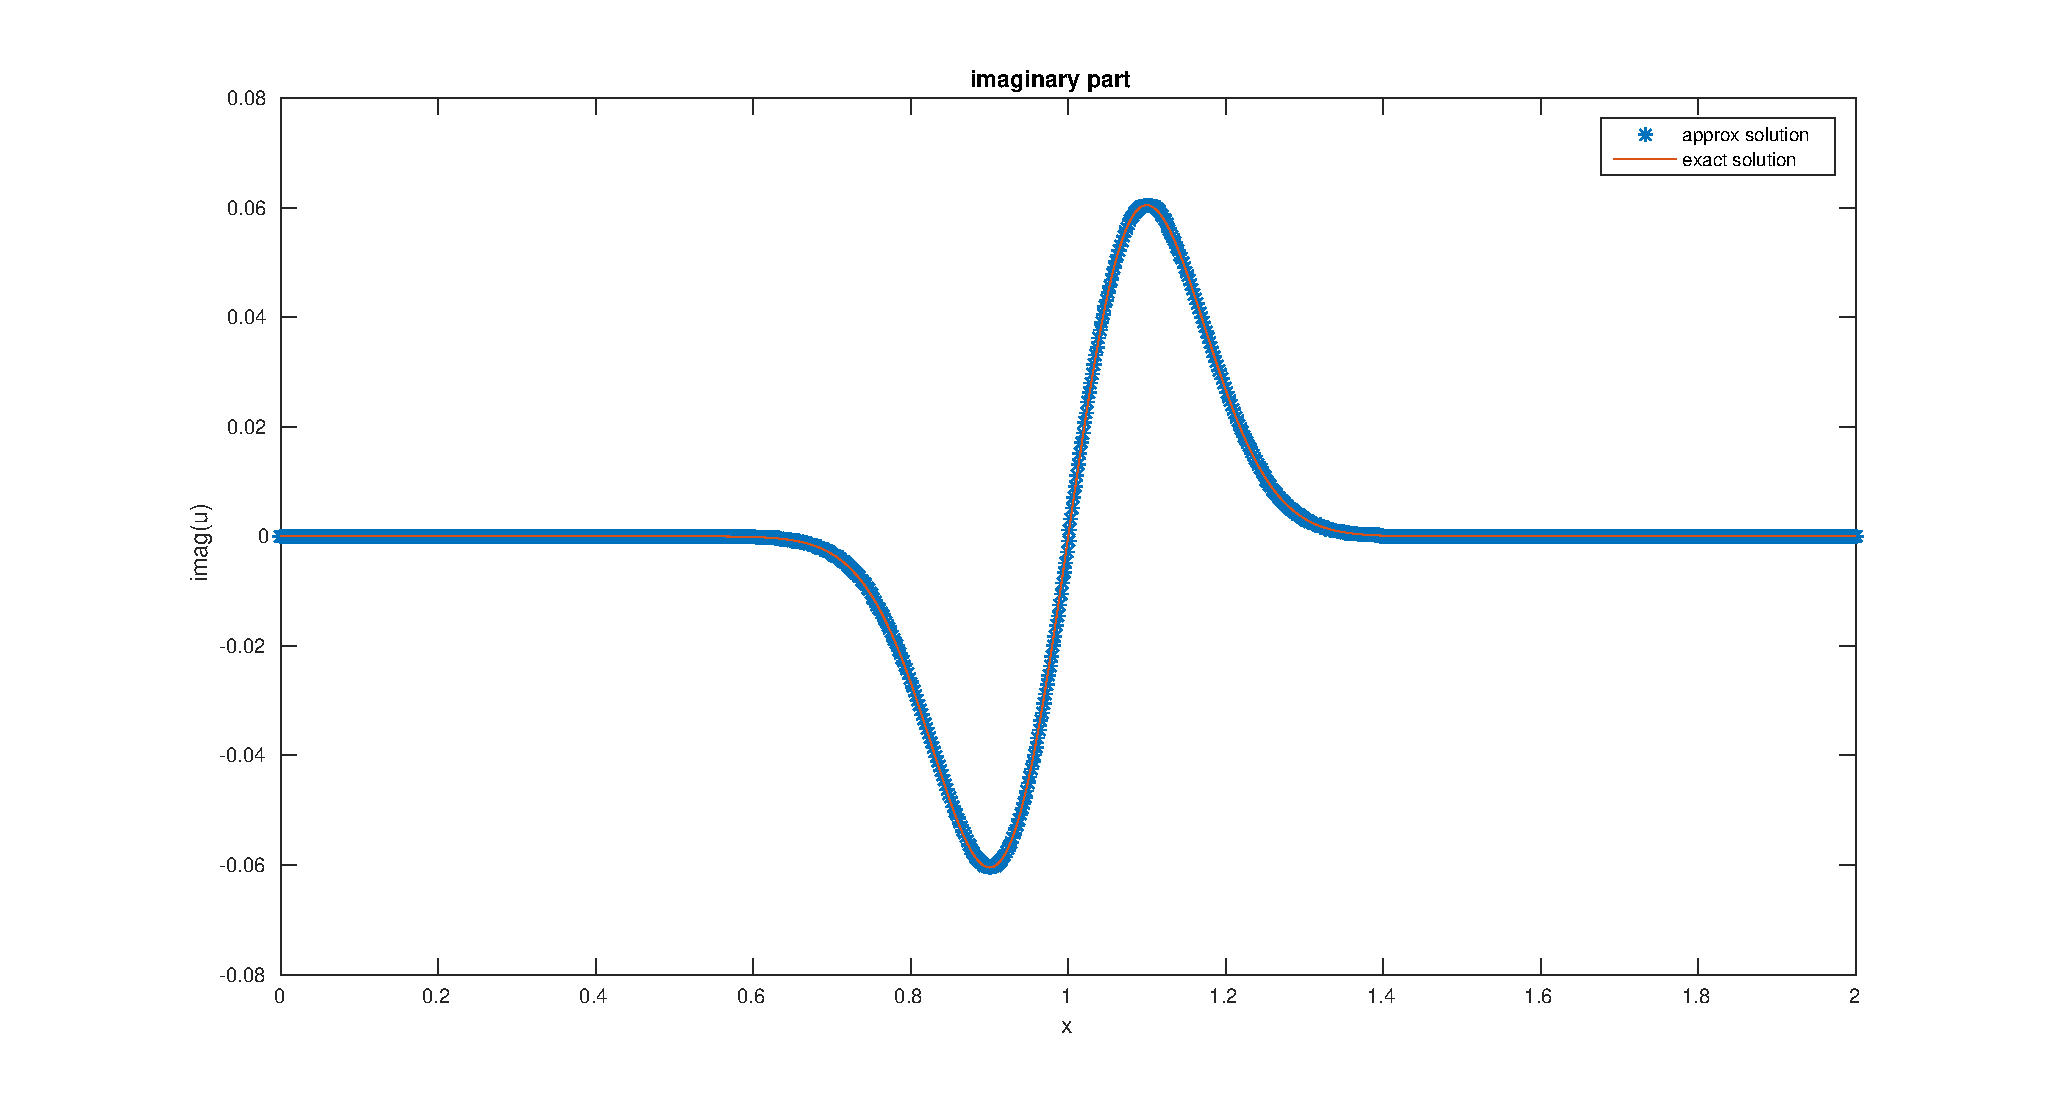
\includegraphics[height=8cm]{Figures/imag_OSTFPM_2_1.eps}\\
		\rule{35em}{0.5pt}
	\caption[OSTFPM imaginary part]{}
\end{figure}

\begin{figure}[htbp]
	\centering
		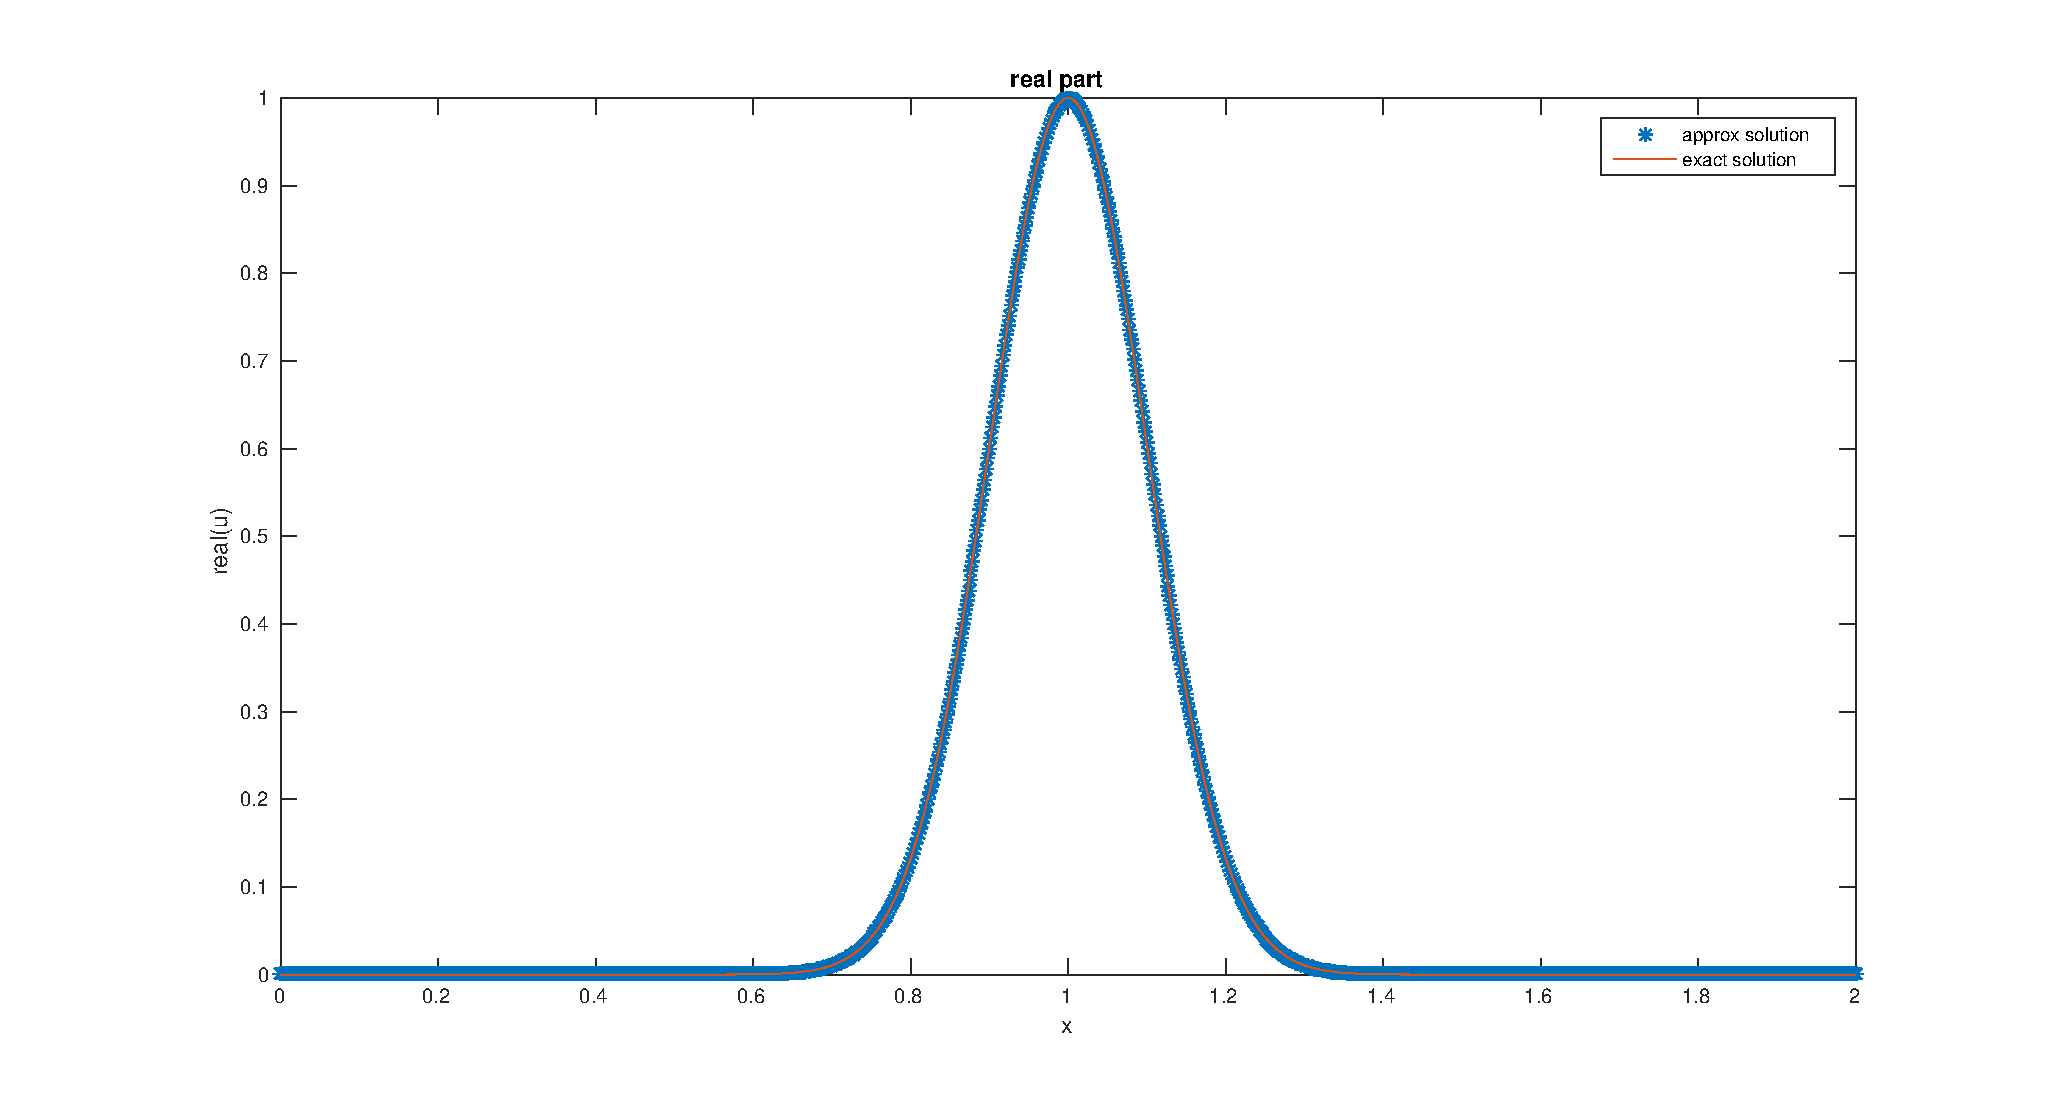
\includegraphics[height=8cm]{Figures/real_OSTFPM_2_1.eps}\\
		\rule{35em}{0.5pt}
	\caption[OSTFPM real part]{}
\end{figure}





